\chapter{Game Analysis for Advanced AI Agents}
\label{advanced_ai_agents}

So far, the only autonomous agent we have seen and used for computing the metrics of Tricolor is the Random Agent. In this chapter, we will analyze some mathematical properties of Tricolor in order to have an overall picture of the AI agents' architecture best suited for the game. Then, we will introduce three advanced agents with the goal of analyzing their performance and decide which one is the best.

\section{Game Complexity}

Defining a simple set of rules in order to determine what move to play at each turn isn't easy for Tricolor because it's a complex combinatorial game. Therefore, any good AI agents for this game will need to explore in some measure the state tree of the game in order to determine the best move \footnote{Ideally, the entire state tree of the game is explored.}. This means the performance of the agents is highly dependent on the average game depth and the average branching factor, as these parameters influence the size of the game state tree.

In the previous chapter ~\ref{game_metrics} where we analyzed the different metrics of Tricolor, we have seen that the average game depth is $\approx 173$ turns and the average branching factor is $\approx 47$. We have also seen that the game tree complexity is $\approx 100^{144}$ and the state tree complexity is $\approx 10^{36}$, which is a lot to explore. Therefore, we introduce game heuristics designed to provide fast and reliable evaluations of positions that cannot be explored further during the search due to time constraints.

\section{Heuristics}
\label{sec:heuristics}

\subsection{First insight}

The goal of the game Tricolor is to make the opponent run out of moves during their turn. In order to achieve this, you need to capture or imprison all of the opponent's pieces \footnote{In theory, a player can run out of legal moves even if he still controls one or more tiles. This happens when the losing player only has stacks fully surrounded by stronger opponent stacks he can't capture. However, such strategies can be neglected when designing heuristics as surrounding weaker opponent stacks doesn't bring a greater advantage than capturing or imprisoning them.}. Therefore, a first solid heuristic is to compare the number of controlled pieces on the board between the players.

\subsection{Second insight}

Capturing and imprisoning opponent pieces but also defending your own requires your stacks to be on stronger tiles \footnote{Red colored tiles triple the power, black doubles it and white has no effect.}. Therefore, a second heuristic is to compare the accumulated power of all the controlled stacks of pieces on the board between the players.

\subsection{Third insight}

Tricolor has a rule specifying that if a player can imprison or capture one or more enemy stacks during their turn, they are forced to play such a move. If we ignored this rule, players could always force any game to end in a draw by stacking at least 3 pieces on any red tile, which will never be captured. This is because the power of such a stack is $3 \times 3 = 9$ and it's impossible to form a stack with power $\geq 10$ in order to at least imprison it. However, because this rule exists, players can make their opponent "break" the power of their stacks placed on red tiles by forcing them to capture nearby pieces. This leads to a game strategy called "Single piece baiting".

To better understand it, let's consider the scenario in Figure \ref{fig:single_pawn_baiting}:

\begin{figure}[h]
    \centering
    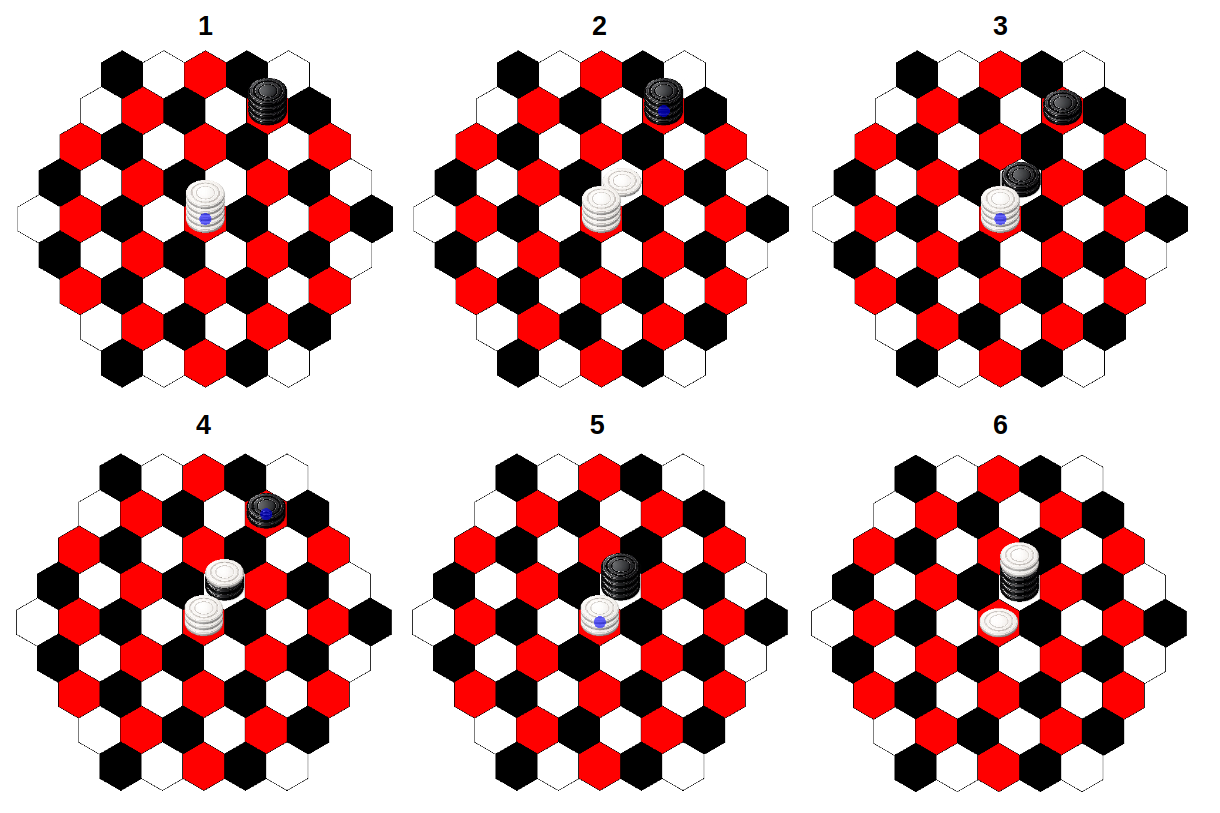
\includegraphics[scale=0.3]{advanced_ai_agents/images/diverse_figures/single_pawn_baiting.png}
    \caption{Figure displaying how the "single piece baiting" strategy used by the white player defeats the powerful stack of the black player.}
    \label{fig:single_pawn_baiting}
\end{figure}

In the scenario presented in Figure \ref{fig:single_pawn_baiting}, the white player (which we will refer to as "White") has a stack of 5 pieces on the red central tile and the black player (which we will refer to as "Black") has a stack of 4 pieces on a red tile close to White. In the second image, White moves a white piece on a white tile, which forces the Black to capture it with at least 2 pieces (because the tile is at distance 2 of their stack). White then repeats the "single piece baiting" strategy until Black runs out of pieces. Finally, in the sixth image, White manages to imprison all of Black's pieces and wins the game \footnote{Notice that White still has one piece left on the initial central tile, which means this strategy also works when both players have stacks of the same size.}. The reason why this strategy works is because the "victim" player (in this case Black) is further away from the contested tile the attacker (in this case White) initially moved its piece to. Now, the question is, can a stack with less pieces win against a stack with more pieces using a "single piece baiting" attack ? The answer is \textbf{no}.\\

\textbf{Proof}:\\
First, we are only interested in positions where both stacks are on red tiles. This is because during a game, good players will try to move their pieces on the red tiles as fast as possible. Also, we are only interested in positions where the tile used as bait has the color white. This is because using a black or red tile as bait will give the defender the advantage of having a better defended stack, which will force the attacker to use even more pieces to continue the attack. By the geometry of the board, which has a hexagonal tiling, we can observe that for any tile, all the tiles at distance 3 have the same color (see Figure \ref{fig:all_tiles_are_red_at_dist_3} as an example). This means a stack on a red tile can't be attacked with a "single piece baiting" attack using a bait tile at distance 3 of the defender. In the best case, such an attack will happen when using a white bait tile at distance two (e.g. in Figure \ref{fig:single_pawn_baiting} where the white bait tile is at distance two of the black stack).

\begin{figure}[h]
    \centering
    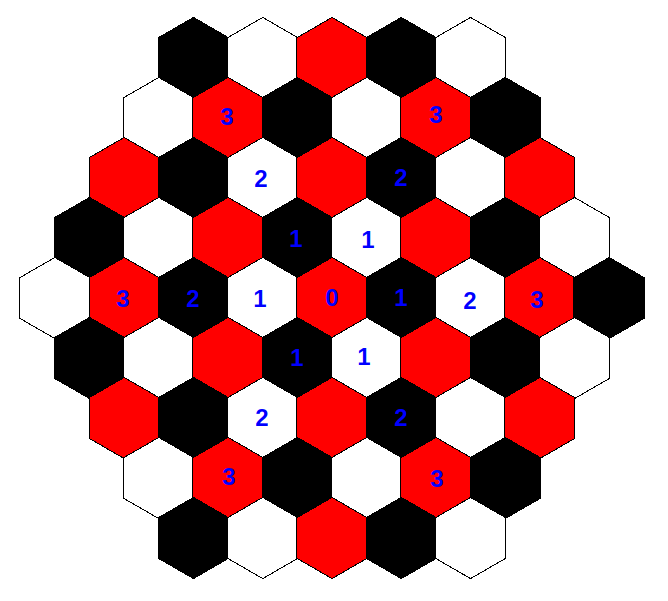
\includegraphics[scale=0.3]{advanced_ai_agents/images/diverse_figures/all_tiles_are_red_at_dist_3.png}
    \caption{Figure showing that all the tiles at distance 3 of the central red tile are also red.}
    \label{fig:all_tiles_are_red_at_dist_3}
\end{figure}

Now that we established the scenarios we are interested in for the "single piece bait" attack, let's show that if the attacker has less pieces than the defender, the attack will never succeed. The following flowchart \ref{fig:schema_single_pawn_bait} proves it by enumerating all the possible moves the attacker has.

\begin{figure}[h]
    \centering
    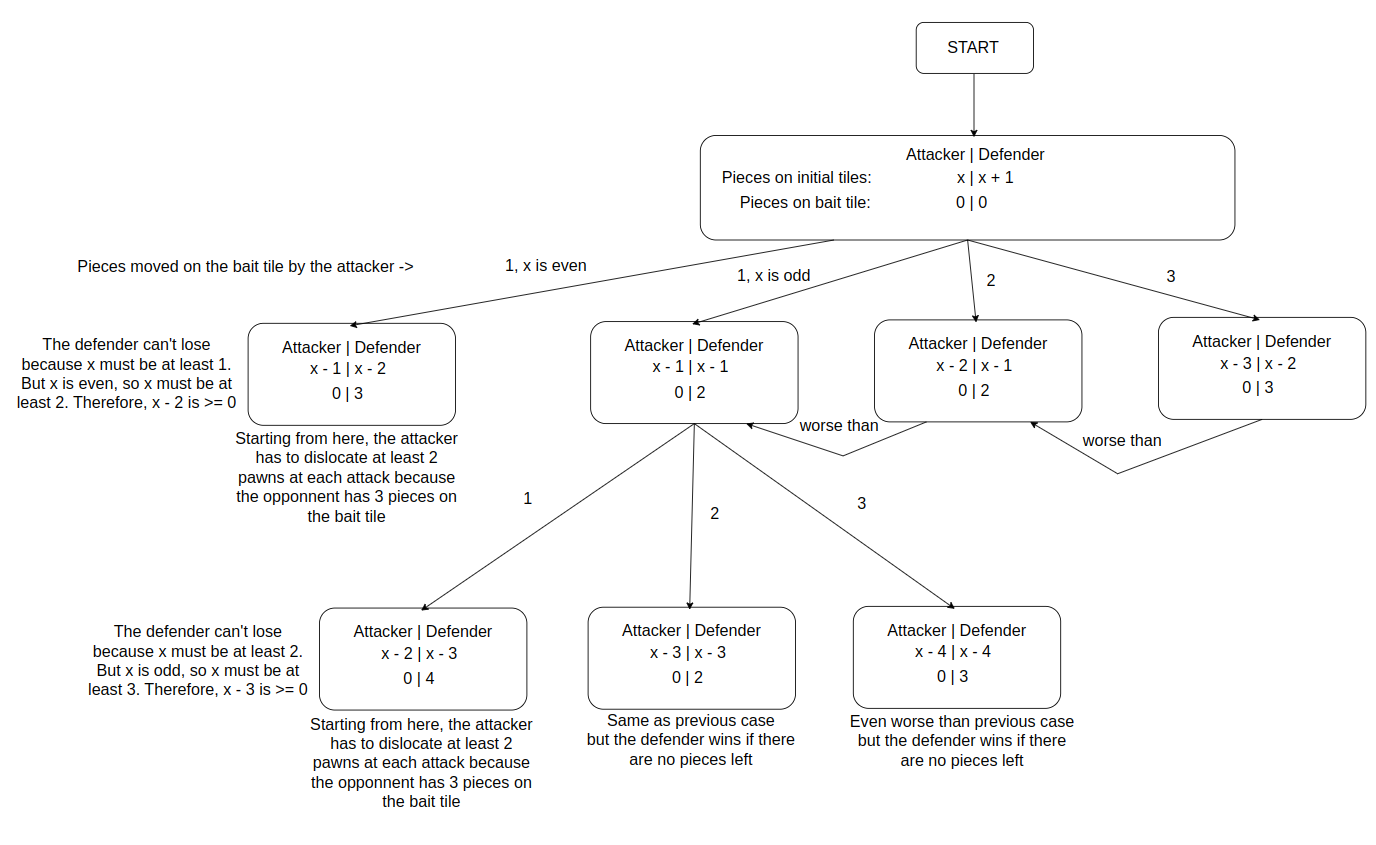
\includegraphics[scale=0.2]{advanced_ai_agents/images/diverse_figures/schema_single_pawn_bait.png}
    \caption{Flowchart of all possible move sequences during a "single pawn bait" attack.}
    \label{fig:schema_single_pawn_bait}
\end{figure}

Finally, a third heuristic is to prioritize stacking pieces on a minimal number of tiles. This is because having a smaller number of big stacks is better than having a bigger number of small stacks. As we just proved earlier, a big stack on a red tile won't be the victim of "single piece bait" attack of a smaller stack, but the opposite is true.

\subsection{Combining the heuristics}

Choosing how to combine these three heuristics is very important because it defines their priority. Analyzing multiple games with different combinations of the two heuristics led to the conclusion that the priorities should be established in the following way:

\begin{itemize}
    \item Comparison of the \textbf{controlled number of pieces} on the board between the players. (Priority 1)
    \item Comparison of the \textbf{accumulated power of all the controlled stacks of pieces} on the board between the players, where the power of a stack is:
    \[ \text{number of pieces}^2 * \text{color} \]
    with the goal of \textbf{preferring taller stacks}. (Priority 2).
\end{itemize}

This choice of priorities is the consequence of the fact that, when mixing the 3 heuristics equally, an AI agent will rather choose to sacrifice pieces only to place other stacks on stronger tiles. This is a bad strategy because it only improves the position in the short term.

\section{Alpha-Beta Agent}

The \textbf{Alpha-Beta Agent} uses the well-known alpha–beta pruning algorithm \cite{alpha_beta} to determine the best move at each turn in one second. This algorithm is an optimization of Minimax by pruning branches not worthy visiting during the search. After the maximum depth is reached and the obtained position is not the end of the game, the heuristic built previously \ref{sec:heuristics} is used to evaluate and score the position.

In addition to the basic alpha-beta algorithm, two improvements are considered:

\begin{itemize}
    \item \textbf{Iterative Deepening} -- a technique that tries all the possible search depths starting from 1, as long as the available time for the player's turn is not over. The improvement is that, instead of having a fixed depth for each turn, the highest possible depth is chosen depending on the current game position. Even if repeating the algorithm for each tested depth wastes time, it is better that fixing a smaller depth for all the played turns.
    \item \textbf{Sorting Actions by Evaluation Score} -- before iterating over the possible actions of a player in a certain position during the search, the list of actions is sorted in decreasing order. This maximizes the chances of pruning future branches earlier in exchange of a small overhead for sorting the lists of actions. 
\end{itemize}

\section{Monte Carlo Tree Search Agent}

The \textbf{Monte Carlo Tree Search Agent} (\textbf{MCTS}) uses the well-known MCTS algorithm to determine the best move at each turn in one second \cite{alpha_beta}. In essence, it consists in running many game simulations starting from the current position and evaluate how good each move is based on the result of each simulation. The algorithm is divided into the four classical steps, with some particularities:

\begin{itemize}
    \item \textbf{Selection} -- the policy used for choosing a child at each fully expanded level of the tree is the \textbf{Upper Confidence bounds applied to Trees} (\textbf{UCT}). The selected child is the one maximizing:
    \[ \frac{w_i}{n_i} + c \cdot \sqrt{\frac{\ln{N}}{n_i}} \],
    where
    \begin{itemize}
        \item $w_i$ is the number of wins for child $i$
        \item $n_i$ is the number of times child $i$ was visited
        \item $N$ is the total visits of the parent
        \item $c$ is the exploration constant. In our implementation, the value of $c$ is chosen to be $\sqrt{2}$, as it was empirically proved to have the best results on average \cite{sqrt_2_constant}.
    \end{itemize}
    \item \textbf{Expansion} -- only one child is expanded at each iteration.
    \item \textbf{Simulation} -- for a game resulting in a win, the score 1 is assigned and 0 otherwise. Draws are not handled.
    \item \textbf{Backpropagation} -- classical implementation.
\end{itemize}

\section{Expert Iteration}

In progress